\graphicspath{{Chapters/ObjEventSelection/Figures/}}
\chapter{Object and Event Selection}
\label{chap:ObjEventSelection}

\section{Electron Selection}
\label{sec:objsel-el}

Electron reconstruction and identification was described in~\sec{reco-el}. Both
central electrons with \modetalt{2.47} and forward electrons are used. In
addition to the identification requirements described in~\sec{reco-el}
additional selection requirements are imposed to select electrons likely to have
originated from \Z\ boson decays and to reject backgrounds. The requirements are
slightly different for the 8 \tev\ analysis compared to the 7 \tev\ analysis,
reflecting the different experimental conditions (such as higher pile-up in
2012) as well as optimisations made in 2012. The electron selection requirements
are summarised in~\tab{objsel-el} are described in more detail below. 

\begin{table}[]
  \centering
%   \vspace*{-1cm}
%\small
\renewcommand\arraystretch{1.07}
  \begin{tabular}{ l  l l }
    \hline\hline 
      Requirement        & 7 \tev\ & 8 \tev\ \\ 
      \hline
      \bf{Central Electron Selection} & \\
      Algorithm             & Standard (with GSF refit)     & Standard \\
      Quality               & Good Data Quality & \it{Same} \\
      ID cut                & \loosePP & \it{Same}       \\
      $\eta$                & $|\eta|<2.47$ & \it{Same} \\
      $E_T$                 & $E_T > 7$ GeV & \it{Same} \\
      \zzero                & $z_0 < 2$ mm & \it{Same} \\
      \dzerosig             & $|d_0|/\sigma(d_0) < 6 $ & \it{Same} \\
      Track isolation       & \ptconetwentylt{0.15} & \it{Same}   \\
      Calorimeter isolation & \etconetwentylt{0.3}          & \it{Not Applied} \\
      Overlap removal       & \multicolumn{1}{p{6cm}}{a) Remove $e$ if $\Delta R < 0.1$ from $\mu$} & \it{Same} \\
                            & \multicolumn{1}{p{6cm}}{b) Remove lowest $E_T$ $e$ in \deltaRlt{0.1} from another $e$} & \it{Same} \\ 
      \hline
      \bf{Forward Electron Selection:} & \\
      Algorithm             & Forward & \it{Same} \\
      Quality               & Good Data Quality & \it{Same}  \\
      ID cut                & Tight & \it{Same} \\
      $\eta$                & $2.50<|\eta|<3.16$ & \it{Same} \\
      $E_T$                 & $E_T > 20$ GeV & \it{Same} \\
      Overlap removal       & \multicolumn{1}{p{6cm}}{Remove if overlaps with central electron or any muon in \deltaRlt{0.1}} & \it{Same}\\
%
      %\bf{Central Electron Selection} & \\
      %Algorithm             & Standard (with GSF refit)     & Standard \\
      %Quality               & \multicolumn{2}{c}{\texttt{(OQ  AND 1446 == 0})} \\
      %ID cut                & \multicolumn{2}{c}{\loosePP}       \\
      %$\eta$                & \multicolumn{2}{c}{$|\eta|<2.47$} \\
      %$E_T$                 & \multicolumn{2}{c}{$E_T > 7$ GeV} \\
      %$z_0$                 & \multicolumn{2}{c}{$z_0 < 2$ mm} \\
      %$d_0$                 & \multicolumn{2}{c}{$|d_0|/\sigma(d_0) < 6 $} \\
      %Track isolation       & \multicolumn{2}{c}{\ptconetwentylt{0.15}}   \\
      %Calorimeter isolation & \etconetwentylt{0.3}          & \it{Not Applied} \\
      %Overlap removal       & \multicolumn{2}{c}{a) Remove $e$ if $\Delta R < 0.1$ from $\mu$} \\
      %                      & \multicolumn{2}{c}{b) Remove lowest $E_T$ $e$ in \deltaRlt{0.1} from another $e$} \\ 
      %\hline
      %\bf{Forward Electron Selection:} & \\
      %Algorithm             & \multicolumn{2}{c}{Forward} \\
      %Quality               & \multicolumn{2}{c}{\texttt{(OQ  AND 1446 == 0)}}  \\
      %ID cut                & \multicolumn{2}{c}{Tight} \\
      %$\eta$                & \multicolumn{2}{c}{$2.50<|\eta|<3.16$} \\
      %$E_T$                 & \multicolumn{2}{c}{$E_T > 20$ GeV} \\
      %Overlap removal       & \multicolumn{2}{p{8cm}}{\centering Remove if overlaps with central electron or any muon in \deltaRlt{0.1}} \\
    \hline \hline
  \end{tabular}
\renewcommand\arraystretch{1}
   \caption{Electron selection requirements.}
   \label{table:objsel-el}
\end{table}

\subsection{Central Electron Selection}

Central electrons, with \modetaclusterlt{2.47} are reconstructed using the
`standard' electron algorithm as described in~\sec{reco-el-reco}.  For 2011
data, the algorithm used was slightly different to the `standard' ATLAS electron
reconstruction as tracks were refitted using a Gaussian-sum filter (GSF) to
account to account for the effect of bremsstrahlung in the inner detector. In
2012 data this became the default reconstruction algorithm. Central electrons
are required to pass the \loosePP\ identification requirements.
%Electrons in the calorimeter ``crack" region $1.37 < |\eta_{cluster}| < 1.52$
%are included, although the efficiency and energy resolution is expected

For electron candidates with 4 or more silicon (SCT and Pixel) hits, the energy
of the electron is taken from the cluster measurement, and the $\eta$ and $\phi$
are taken from the track measurement (this requirement is automatically
satisfied for electrons passing the \loosePP\ identification requirements). For
electron candidates with fewer than 4 silicon hits, all electron parameters are
taken directly from the cluster. In both cases, the cluster $\eta$ and $\phi$
are used for the $\eta$ requirement and for overlap removal. Using the energy
and direction defined in this way, the electron candidates are required to have
\etgt{7}, where \et\ is defined as $E\sin(\theta)=E/\cosh(\eta)$. 

A small number of the front-end boards of the LAr calorimeter were
inactive in 2011 and 2012; the exact number varied with time as some were
repaired whilst other developed faults. Additionally, a number of individual
cells were masked in the readout (i.e. have their energy set to zero) due to
consistently producing high noise or failing to give a readout. There are also
regions where the High-Voltage supply to the LAr is faulty. Electrons are
rejected if they fall into a region of $\eta, \phi$ space consistent with the
presence of a dead front-end board in the first or second sampling layer, the
presence of a dead HV region affecting all three samplings, or the presence of a
masked cell in the core of the cluster.

To ensure that the candidates come from the primary vertex (defined as the
vertex that has the highest $\sum{\pt^2}$ of associated tracks), the
longitudinal impact parameter \zzero\ of the electron track with respect to the
primary vertex must be less than 2 mm for data collected in 2011. For 2012 data,
the requirement is \zzerosintheta $<$ 0.5 mm. The \intro{unbiased} impact
parameter is used; obtained by refitting the vertex without the track in
question, then calculating the impact parameter with respect to this refitted
vertex, thus removing the pull of the track from the vertex fit.  The transverse
impact parameter \dzero\ must have a significance (\dzero\ divided by the error
on its measurement, \dzerosig) less than 6. This helps reduce backgrounds,
particularly from decays of pions and kaons in jets to electrons, since these
decays will occur further from the interaction point giving larger impact
parameters.

Isolation requirements are applied to reduce the backgrounds from jets being
misidentified as electrons, or from electrons from decays in jets, collectively
referred to as \intro{background electrons}. Such background electrons will
typically have many tracks surrounding their track in the tracker, and be
surrounded by large energy deposits in the calorimeter from other particles in
the jet. \intro{Track Isolation} requirements are imposed, requiring that the
sum of the \pt\ of tracks surrounding the electron's track in a cone of
\deltaRlt{0.2} be less than 15\% of the electron's \pt, i.e.
\ptconetwentylt{0.15}. Tracks included in the calculation are required to have
\ptgt{0.4}, have impact parameters consistent with the same vertex as the
electron and have at least 9 silicon hits, thus ensuring good track quality and
purity. The impact parameter requirement means that this variable is insensitive
to pileup as most tracks from other (pileup) vertices are excluded.

Additionally, for the 2011 data, a calorimeter isolation requirement is imposed.
This is defined as the sum of calorimeter cell energies in a cone of
\deltaRlt{0.2} around the barycentre of the electron cluster, excluding a 5x7
grid of cells in the centre of the cone (which are assumed to be due to the
electron). Cells from both the EM and hadronic calorimeters are included. The
requirement is that the sum of such energies be less than 30\% of electron \et,
i.e. \etconetwentylt{0.3}.  This variable is particularly sensitive to pileup,
as pileup events tend to deposit additional energy isotropically throughout the
detector, thus increasing the energy in the isolation cone. A correction
parameterised by the number of vertices reconstructed in the event is applied to
correct the isolation variable for extra energy due to pileup.  Additional
corrections are applied to correct for leakage of the electron's energy out of
the core cells of the cone, which tends to increase with \pt. Calorimeter
isolation requirements were not applied in 2012.

Electrons closer than \deltaRlt{0.1} to a muon which passes the muon selection
requirements (see~\sec{objsel-mu}) are rejected. If two selected electrons
overlap within \deltaRlt{0.1}, the lower-\et\ electron is removed, although in
the case of a central electron overlapping with a forward electron, which could
occur near the edge of the tracker, the central electron would take precedence.

\subsection{Forward Electron Selection}

Electrons reconstructed using the forward electron reconstruction algorithm are
used to to extend the pseudo-rapidity coverage beyond the limit of the tracker,
\modetaeq{2.5}. Only electrons falling in the EMEC region are used, with
pseudo-rapidity \modetaclusterbetween{2.5}{3.16}.  Since the lack of tracking makes it
harder to reject hadronic and photonic fakes, these electrons are required to
pass tighter identification requirements: ``Forward Tight''. Since forward
electrons lack a track measurement, it is impossible to determine their charge,
and of course impossible to apply track isolation and track parameter cuts.
Forward electrons are required to have \etgt{20}; this higher energy requirement
is motivated by the difficulty of measuring reconstruction and identification
efficiencies in data below this energy and by the higher hadronic and photonic
backgrounds at low energy.
%For this reason a tighter calorimeter isolation requirement is applied: the sum
%of the calorimeter transverse energy in a cone of $\Delta R = 0.3$ around the
%electron, removing the electron energy, must be less than 10\% of the electron
%energy.

\begin{figure}[h]
\centering
	\subfigure[]{
            \includegraphics[width=0.47\textwidth]{ObjSel/h_4l_ElEtCone20_log}
        }
	\subfigure[]{
            \includegraphics[width=0.47\textwidth]{ObjSel/h_4l_ElPtCone20_log}
        }
	\subfigure[]{
            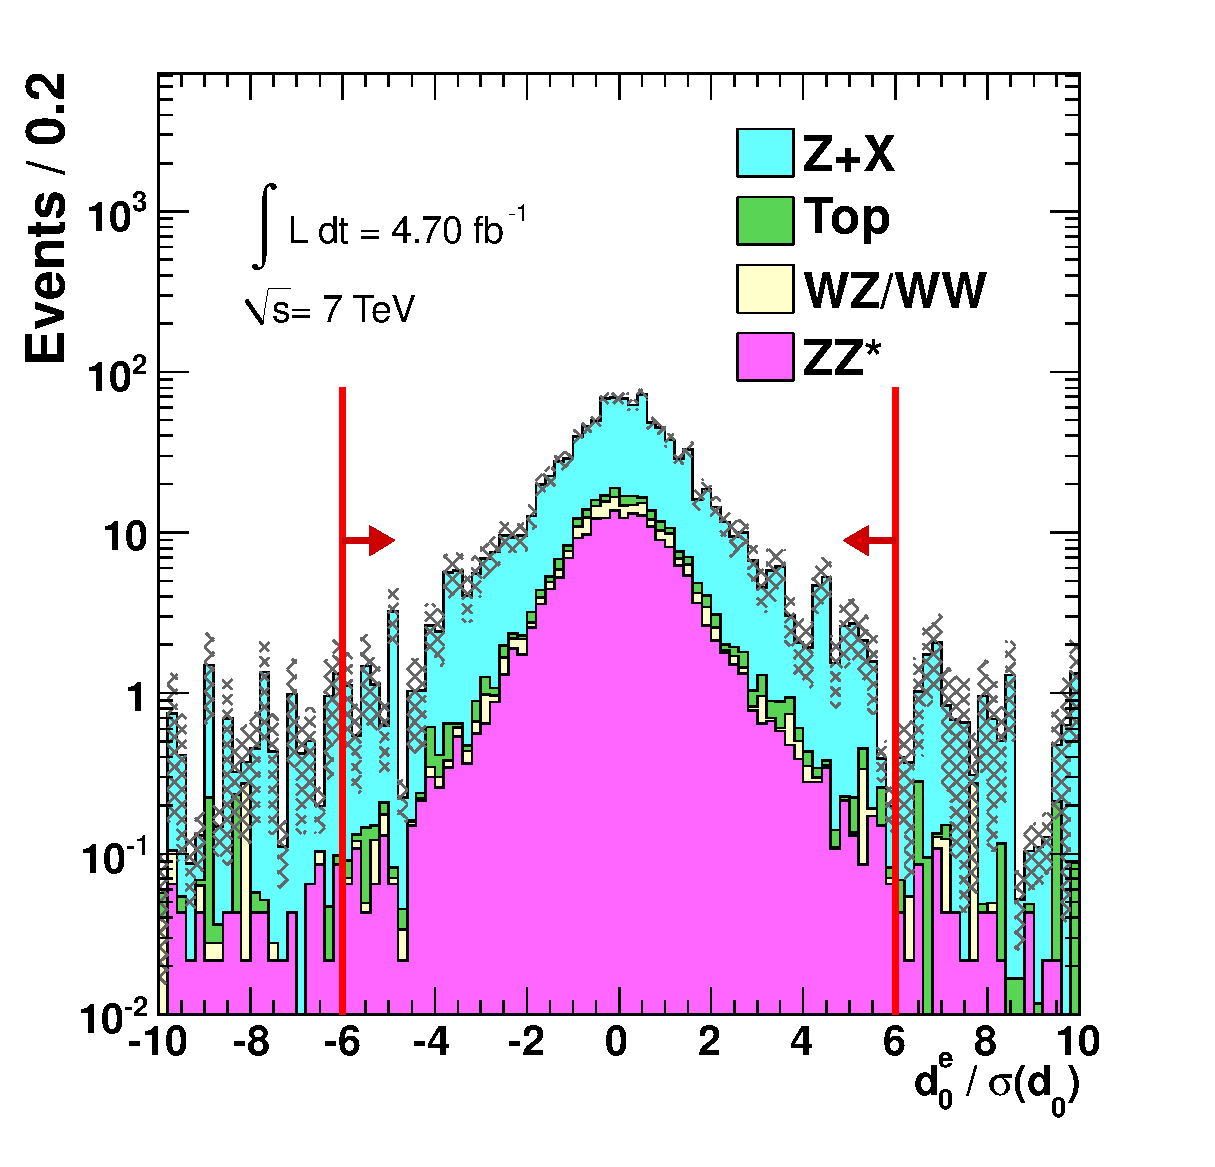
\includegraphics[width=0.47\textwidth]{ObjSel/h_4l_Electron_d0Sig_log}
        }
\caption[ ]{}
\label{fig:objsel-el}
\end{figure}

\section{Muon Selection}
\label{sec:objsel-mu}

\begin{table}[]
  \centering
%   \vspace*{-1cm}
\small
\renewcommand\arraystretch{1.07}
  \begin{tabular}{ l  l l }
    \hline\hline 
      Requirement        & 7 \tev\ & 8 \tev\ \\ 
      \hline
      \bf{Central Muons} & \\
      Algorithm             & \staco                        & \same \\
      Type                  & Combined or Segment Tagged    & \same \\
      $\eta$                & $|\eta|<2.5$                  & \same \\
      $p_T$                 & $p_T > 7$ GeV                 & \same \\
      ID Track Quality      & & \\
       - B Layer Hits       & $\geq 1$                      & \same \\
       - Pixel Hits         & $\geq 2$                      &  $\geq 1$\\
       - SCT Hits           & $\geq 6$                      &  $\geq 5$\\
       - Silicon `Holes'    & $<3$                          & \same \\
       - TRT                & \multicolumn{1}{p{5cm}}{\raggedright
                                {\bf If \modetalt{1.9}:} 
                                Require $n_{hits}+n_{outliers}>5$ 
                                and $n_{outliers}/(n_{hits}+n_{outliers})<0.9$}
                                                            & \multicolumn{1}{p{5cm}}{\raggedright
                                                                {\bf If \modetabetween{0.1}{1.9}:} 
                                                                Require $n_{hits}+n_{outliers}>5$ 
                                                                and $n_{outliers}/(n_{hits}+n_{outliers})<0.9$} \\
                            & \multicolumn{1}{p{5cm}}{\raggedright
                                {\bf If \modetagt{1.9}:} 
                                If $n_{hits}+n_{outliers}>5$ 
                                require $n_{outliers}/(n_{hits}+n_{outliers})<0.9$} 
                                                            & \multicolumn{1}{p{5cm}}{\raggedright
                                                                {\bf If \modetagt{1.9} or \modetalt{0.1}:} 
                                                                If $n_{hits}+n_{outliers}>5$ 
                                                                require $n_{outliers}/(n_{hits}+n_{outliers})<0.9$} \\
      \zzero                & $|z_0| < 2$ mm & $|z_0\sin(\theta)| < 0.5$ mm \\
      \dzerosig             & $|d_0|/\sigma(d_0) < 3.5 $    & \same \\
      Track isolation       & \ptconetwentylt{0.15}         & \same   \\
      Calorimeter isolation & \etconetwentylt{0.3}          & \it{Not Applied} \\
      \hline
      \bf{Forward Muons} & \\
      Algorithm             & \staco                        & \same \\
      Type                  & Combined or Stand-Alone       & \same \\
      $\eta$                & \modetabetween{2.5}{2.7}      & \same \\
      $p_T$                 & $p_T > 10$ GeV                & \same \\
      Calorimeter isolation & \etconetwentylt{0.15}         & \same \\
      % This is a cut that is automatically satisfied by combined
      %MS Track Quality      & Hits in all 3 stations       & \same \\
       \multicolumn{3}{c}{\it \underline{Additional requirements for Combined Muons}} \\
      ID Track Quality      &                               &  \\
       - B Layer Hits       & $\geq 1$                      & \same \\
       - Pixel Hits         & $\geq 2$                      & $\geq 1$\\
       - SCT Hits           & $\geq 4$                      & $\geq 3$\\
       - Silicon `Holes'    & $<3$                          & \same \\
      \zzero                & $|z_0| < 2$ mm                & $|z_0\sin(\theta)| < 0.5$ mm \\
      \dzerosig             & $|d_0|/\sigma(d_0) < 3.5 $    & \same \\
      \hline
      \multicolumn{2}{l}{\bf Calorimeter Tagged Muons} & \\
      Type                  & Calorimeter Tagged            & \same \\
      $\eta$                & \modetalt{0.1}                  & \same \\
      $p_T$                 & $p_T > 20$ GeV                & \same \\
      Quality               & Calorimeter Muon ID Cuts      & \same \\
      % This is a cut that is automatically satisfied by combined
      %MS Track Quality      & Hits in all 3 stations       & \same \\
      Overlap removal       & \multicolumn{1}{p{5cm}}{Remove 
                              if overlaps with a central 
                              muon in \deltaRlt{0.1}}  & \it{Same}\\
      \multicolumn{3}{c}{\it ID Track Quality, Track Isolation, Calorimeter
                                Isolation, \zzero, \dzerosig\ as central muons} \\
      %ID Track Quality      & As Central Muons              &  \\
      %Calorimeter isolation & \etconetwentylt{0.3}         & \same \\
      %Track isolation       & \ptconetwentylt{0.15}         & \same   \\
      %$z_0$                 & $|z_0| < 2$ mm                & $|z_0\sin(\theta)| < 0.5$ mm \\
      %$d_0$                 & $|d_0|/\sigma(d_0) < 3.5 $    & \same \\
                                                            
%
      %\bf{Central Electron Selection} & \\
      %Algorthim             & Standard (with GSF refit)     & Standard \\
      %Quality               & \multicolumn{2}{c}{\texttt{(OQ  AND 1446 == 0})} \\
      %ID cut                & \multicolumn{2}{c}{\loosePP}       \\
      %$\eta$                & \multicolumn{2}{c}{$|\eta|<2.47$} \\
      %$E_T$                 & \multicolumn{2}{c}{$E_T > 7$ GeV} \\
      %$z_0$                 & \multicolumn{2}{c}{$z_0 < 2$ mm} \\
      %$d_0$                 & \multicolumn{2}{c}{$|d_0|/\sigma(d_0) < 6 $} \\
      %Track isolation       & \multicolumn{2}{c}{\ptconetwentylt{0.15}}   \\
      %Calorimeter isolation & \etconetwentylt{0.3}          & \it{Not Applied} \\
      %Overlap removal       & \multicolumn{2}{c}{a) Remove $e$ if $\Delta R < 0.1$ from $\mu$} \\
      %                      & \multicolumn{2}{c}{b) Remove lowest $E_T$ $e$ in \deltaRlt{0.1} from another $e$} \\ 
      %\hline
      %\bf{Forward Electron Selection:} & \\
      %Alogirthm             & \multicolumn{2}{c}{Forward} \\
      %Quality               & \multicolumn{2}{c}{\texttt{(OQ  AND 1446 == 0)}}  \\
      %ID cut                & \multicolumn{2}{c}{Tight} \\
      %$\eta$                & \multicolumn{2}{c}{$2.50<|\eta|<3.16$} \\
      %$E_T$                 & \multicolumn{2}{c}{$E_T > 20$ GeV} \\
      %Overlap removal       & \multicolumn{2}{p{8cm}}{\centering Remove if overlaps with central electron or any muon in \deltaRlt{0.1}} \\
    \hline \hline
  \end{tabular}
   \caption{Muon selection requirements.}
   \label{table:objsel-mu}
   \renewcommand\arraystretch{1}
\end{table}

Muon reconstruction was described in~\sec{reco-mu}. Three distinct categories of
muons are used in this analysis: `central' muons with \modetalt{2.5} and
`forward' muons with \modetabetween{2.5}{2.7}, both reconstructed with the
\staco\ algorithm, and calorimeter tagged muons with \modetalt{0.1},
reconstructed without using the muon spectrometer. As for electrons, additional
selection requirements are imposed to select muons likely to have originated from
\Z\ boson decays and to reject backgrounds. The muon selection requirements are
summarised in~\tab{objsel-mu} are described in more detail below. 

\subsection{Central Muon Selection}

Central muons must be either Combined (with a full MS and ID track) or Segment
Tagged (with a full ID track but only an MS track segment), and have $\pt>7$ GeV
and \modetalt{2.47}.

As for electrons, track and calorimeter isolation requirements are imposed to
reject backgrounds. In the case of muons this is mainly from heavy flavour
decays in jets and `punch-through' of hadrons into the muon spectrometer.  The
track isolation is defined in the same way as for electrons, and as for
electrons the requirement
is \ptconetwentylt{0.15}.  The calorimeter isolation variable is defined in a
similar way as for electrons, however the size of the `core' deposit of energy
attributed to the muon is smaller than in the case of electron isolation, and
varies by calorimeter component depending on the expected muon energy deposition
pattern (e.g. a single cell in the EM pre-sampler and 3x3 grid of cells in the second
layer of the EM calorimeter). The calorimeter isolation requirement is
\etconetwentylt{0.3}, and as for electrons is only applied to the 2011 data.

To ensure that the candidates come from the primary vertex, the magnitude
of the longitudinal impact parameter with respect to the primary vertex,
$|z_0|$ must be less than 2 mm for data taken in 2011. For data taken in 2012,
the requirement is $|z_0\sin(\theta)|<0.5$ mm. The transverse impact parameter
significance, \dzerosig is required to be less than 3.5. The selection for
muons is tighter than for electrons since because muons do not emit \brem\ to
the same extent as electrons the track fit is improved, and so the resolution of
the impact parameter is improved, so tighter requirements 
can be made whilst maintaining high signal efficiency.

The inner detector tracks associated with central muons must have a minimum
number of hits in each silicon sub-detector to ensure good track quality. For
2011 data the requirements are: at least 1 hit in the B-layer, $2$ in all Pixel
layers, $6$ in the SCT, and less than 3 holes (no hit in a layer crossed by the
track) in all silicon layers. For all silicon hit conditions, dead sensors count
as hits observed, not as holes.  Finally, a pseudo-rapidity dependent condition
on TRT hits and outliers is applied to ensure that the TRT extension of the
track is successful within the $\eta$ acceptance of the TRT (TRT hits can be
associated as outliers when the extension is not successful): for $|\eta| <
1.9$, require $\mathrm{hits}+\mathrm{outliers} > 6$ and $\mathrm{outliers} < 0.9
\times (\mathrm{outliers}+\mathrm{hits})$; for $|\eta| > 1.9$, if
$\mathrm{hits}+\mathrm{outliers} > 6$, require $\mathrm{outliers} < 0.9 \times
(\mathrm{outliers}+\mathrm{hits})$. For data taken in 2012, the
requirements are slightly loosened in order to recover efficiency losses in 2012
data; this was not found to increase the misidentification rate significantly;
see~\tab{objsel-mu} for details of the changes.

\subsection{Forward Muon Selection}

Muons in the region \modetabetween{2.5}{2.7} are required to have a full muon
spectrometer track with hits in each station of the spectrometer and have
\ptgt{10}. Although the
inner detector only extends to \modetaeq{2.5}, the complicated nature of the
magnetic field makes it possible for some muons up to \modetalt{2.6} to be
combined with an ID track, forming `Combined' muons; those that do not have an
ID track are termed Stand Alone.  In data reconstructed in 2012 muons without a
full ID track may be combined with pixel detector `tracklets' up to
\modetalt{2.65}. Such `Silicon Associated' muons benefit from improved vertex
parameter estimation, but are otherwise treated as Stand Alone. 

Since not all forward muons
have tracks, a track isolation requirement is not applied; instead a tighter calorimeter isolation
requirement is applied to forward muons: \etconetwentylt{0.15}. This is applied
to both 2011 and 2012 data.

For forward muons with an ID track, a set of ID track quality
cuts are applied to the number of hits in the silicon detectors, similar to the
cuts for central muons but slightly looser. For data taken in 2011
the requirements are: at least 1 hit in the B-layer, $2$ in all Pixel layers,
$4$ in the SCT, and less than 3 holes (no hit in a layer crossed by the track)
in all silicon layers. No cut is applied to the number of TRT hits. As for
central muons, the requirements were relaxed slightly for 2012 data.
Additionally, forward muons with an ID track are required to satisfy the same
\zzero\ and \dzerosig\ requirements as central muons.

\subsection{Calorimeter Tagged Muon Selection}

Calorimeter tagged muons are used to recover efficiency at \modetalt{0.1} where
there is a gap in the muon-spectrometer. They must have \ptgt{20}. The reason
for this higher \pt\ requirement is the higher level of fakes from jets and
electrons at low \pt, and the difficulty of measuring the identification
efficiency for $\pt<20\gev$. They are required to pass either the cut or
likelihood based calorimeter tagged muon identification requirements described
in~\sec{reco-mu-reco}, and are not selected if they overlap with a selected
central muon within \deltaRlt{0.1}. Calorimeter tagged muons must satisfy the
same track and calorimeter isolation, ID track quality, \zzero\ and \dzerosig\
requirements as central muons.

\begin{figure}[h]
\centering
	\subfigure[]{
            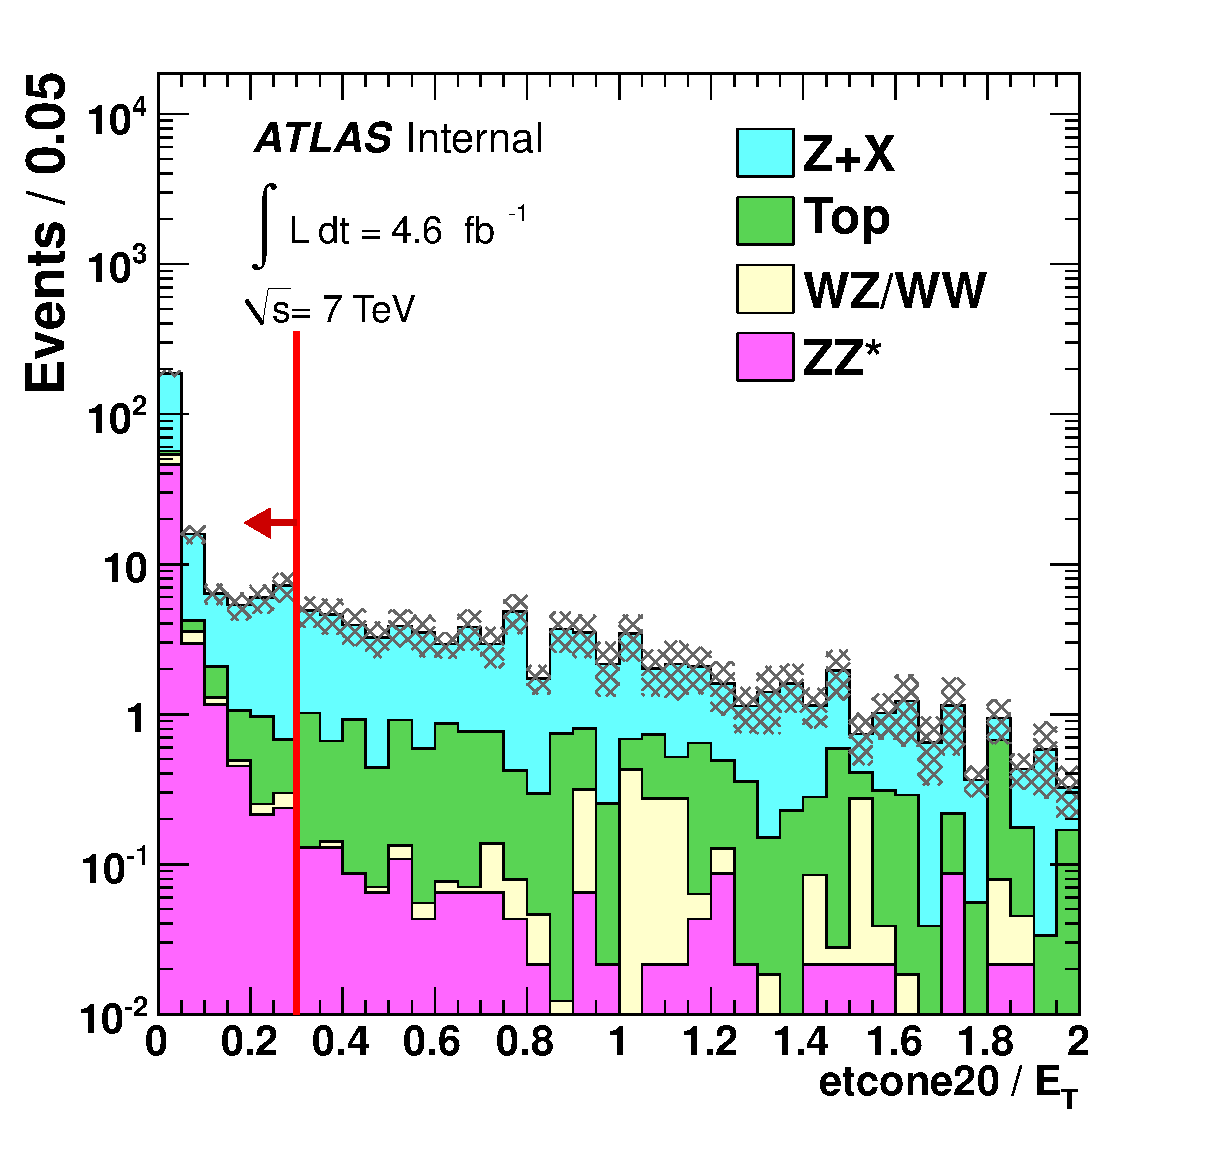
\includegraphics[width=0.47\textwidth]{ObjSel/h_4l_MuEtCone20_log}
        }
	\subfigure[]{
            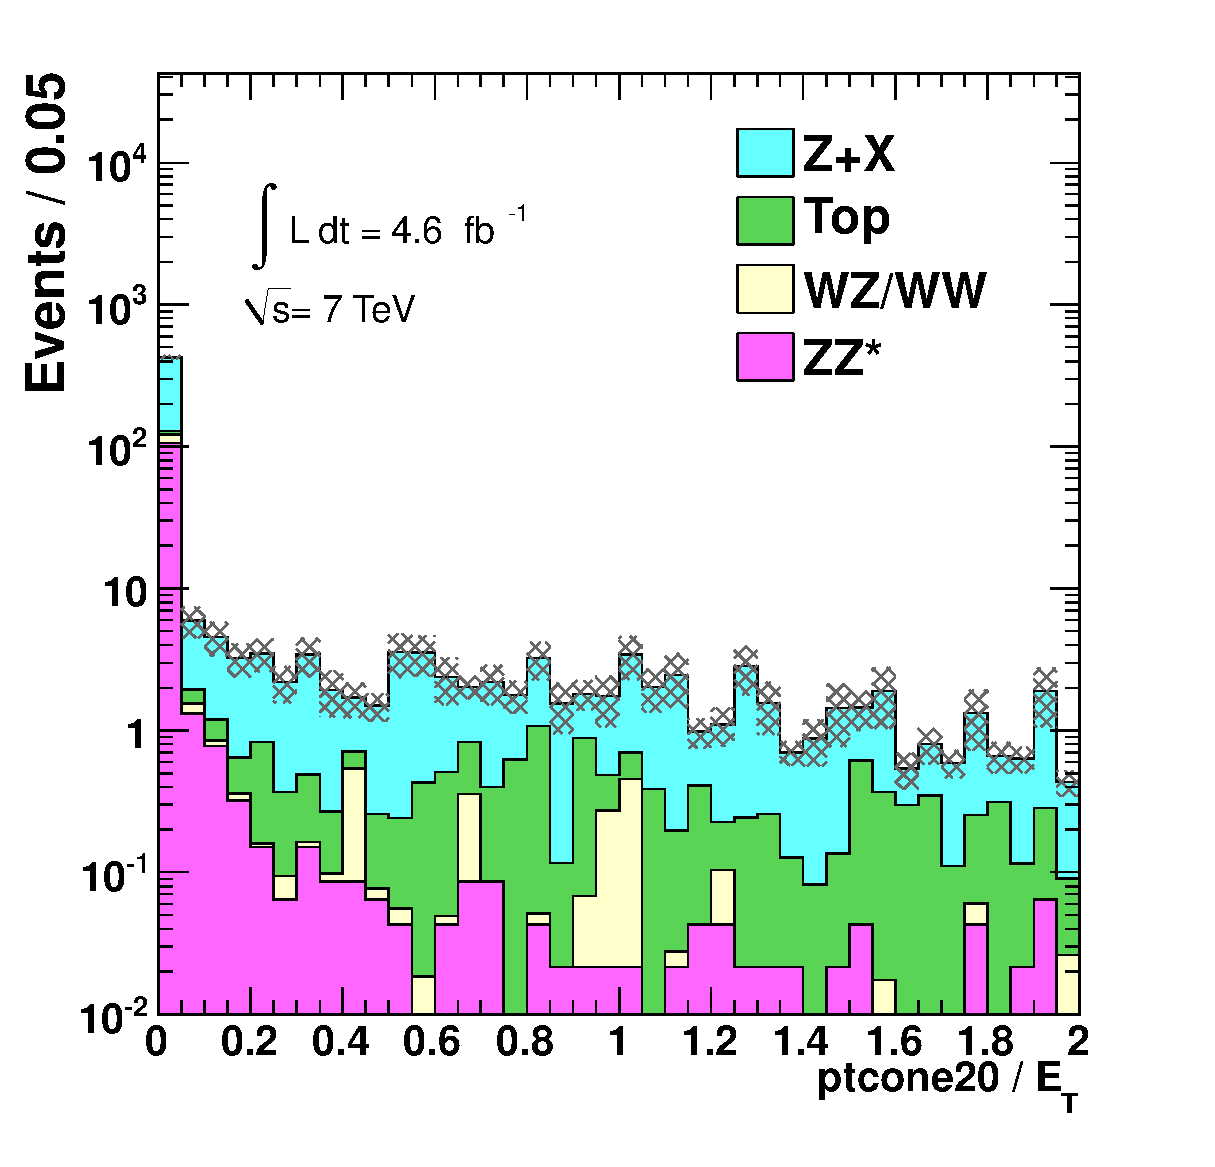
\includegraphics[width=0.47\textwidth]{ObjSel/h_4l_MuPtCone20_log}
        }
	\subfigure[]{
            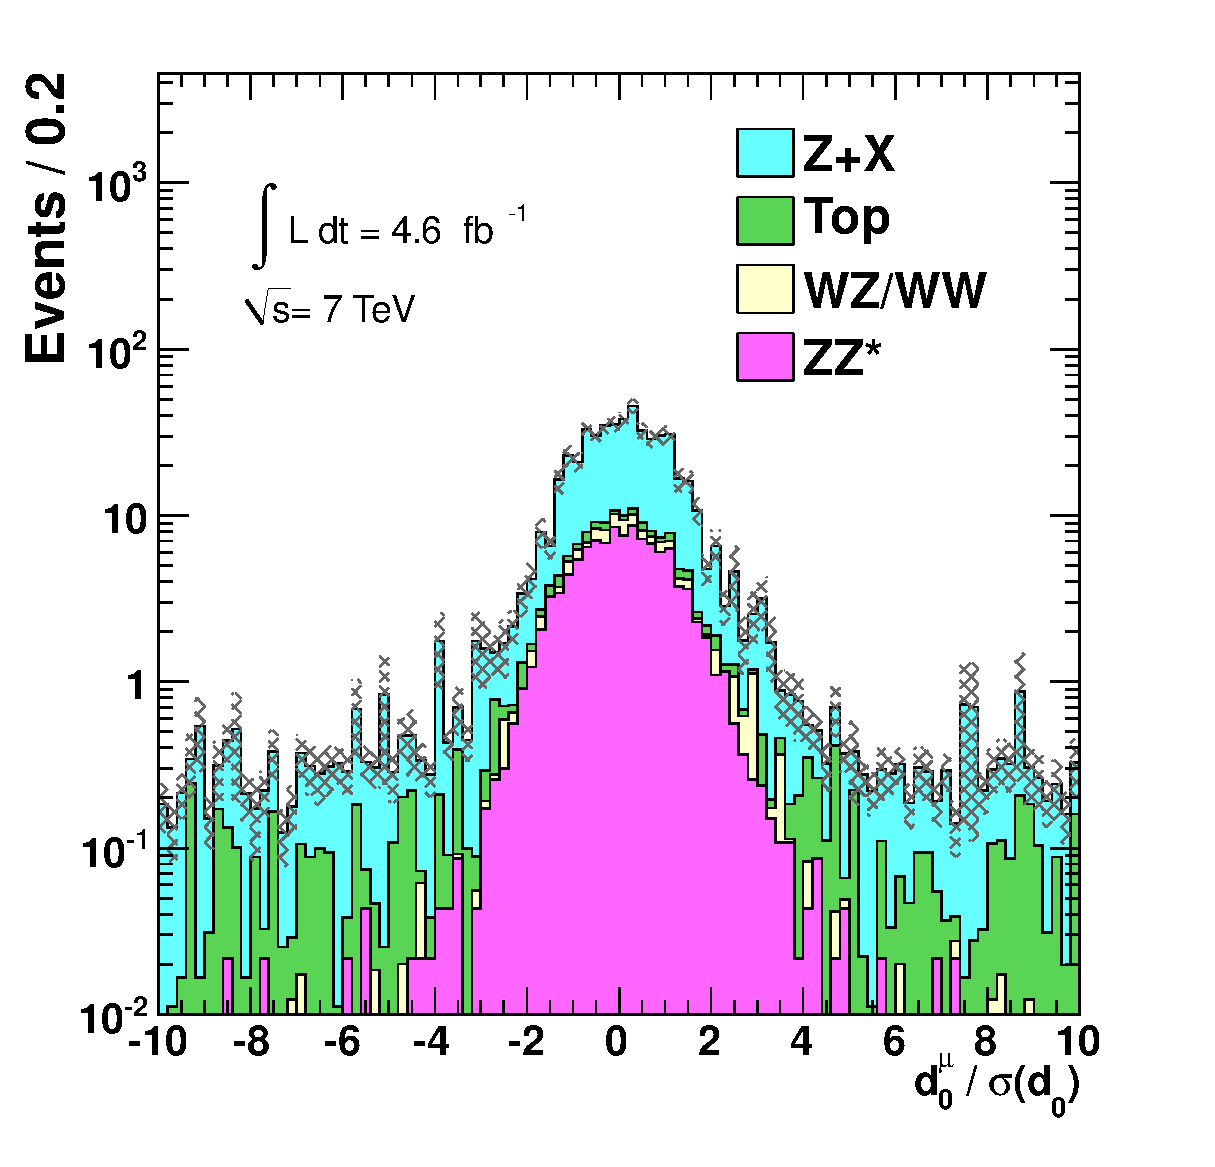
\includegraphics[width=0.47\textwidth]{ObjSel/h_4l_Muon_d0Sig_log}
        }
\caption[ ]{}
\label{fig:objsel-mu}
\end{figure}

%\section{Jet Selection}

\section{Triggers}
\label{sec:triggers}

\ZZ\ candidate events in are pre-selected using the lowest threshold unprescaled single-electron or
single-muon triggers, as descried in Section~\ref{sec:reco-el-trigger}
and~\ref{sec:reco-mu-trigger}. The trigger thresholds were progressively
increased with time as the instantaneous luminosity delivered by the LHC
increases. For the \eemm\ final state, the event may be selected using either
the electron trigger or the single muon trigger. The triggers used and the
associated luminosity are shown in~\tab{objSel-trigger-el} for the electron
trigger and~\tab{objSel-trigger-mu} for the muon trigger.

\begin{table}[htbp]
\begin{center}
\begin{tabular}{lcccc}
\hline \hline
Period & Trigger & \pt\ threshold (GeV) & Int. Luminosity (\ifb) & Notes \\
\hline
{ \bf 2011 } & & & & \\
B - I & \texttt{e20\_medium} & 20 & & \\
J - K & \texttt{e22\_medium} & 22 & & \\
L - M & \texttt{e22vh\_medium1} & 22 & & Variable L1 thresholds; hadronic
\hline
{ \bf 2012 } & & & & \\
A - I & \texttt{e20\_medium} & 20 & & \\
J - K & \texttt{e22\_medium} & 22 & & \\
L - M & \texttt{e22vh\_medium1} & 22 & & Variable L1 thresholds; hadronic
leakage cut; Reoptimised ID cuts.\\
leakage cut; Reoptimised ID cuts.\\
\hline
\end{tabular}
\end{center}
\caption{Single electron triggers used in the different data taking periods}
\label{table:objSel-trigger-el}
\end{table}

The events passing the pre-selection are required to possess a 
%leading
``trigger-matched lepton'', i.e., a lepton that is within $\dR<0.1$ of the
triggered object.  At least one trigger-matched lepton must have 
$\pt>25$ GeV and $|\eta|<2.47$ (if it is an electron) or $\pt>20$ GeV
and $|\eta|<2.4$ (if it is a muon). 

%	Due to the presence of three leptons with large transverse momentum
%	the trigger efficiencies for $ZZ$ events is higher than the single
%	lepton trigger efficiency. 

The scale factors to account for the mis-modeling of the single-lepton
trigger efficiency in the MC with respect to the data have been
derived using the tag-and-probe method (T\&P) on $Z\rightarrow \ll$
events. The statistical uncertainty on the trigger efficiency is obtained
from MC.

The scale factors are applied to leptons forming the $\Z$ candidate which
match to a trigger object as described above.
The scale factor depends on the lepton flavor and $\pt$ of the individual leptons. It is calculated 
according to equation~(\ref{eq:triggerEffSF}) where $N_l$ is the number of leptons
matching to a trigger object,
$\epsilon_{Data,l_n}$ is the trigger efficiency determined with T\&P from 
data for a single lepton flavor of lepton $l_n$, and $\epsilon_{MC,l_n}$ is
the trigger efficiency determined with T\&P from MC. 

\begin{equation}\label{eq:triggerEffSF}
  SF =  { \frac{ {1 - \prod_{n=1}^{N_l} (1 - \epsilon_{Data,l_n})}} {1 - \prod_{n=1}^{N_l} (1 - \epsilon_{MC,l_n})} }
\end{equation}

The systematic uncertainty associated with the scale factors for
muon triggers is $0.2\%$~\cite{muonPG_EPS}.
The
uncertainty associated with the electron trigger is $1\%$, which is given
by the e-gamma performance group~\cite{egammaPG_EPS}. 

%The efficiency corrected with the scale factor 
%will be calculated, and
%is 
%compared with the scale factor uncertainty. If the correction is much smaller
%than the scale factor uncertainty, a correction will not be used. The maximum
%systematic uncertainty in the trigger efficiency is expected to be no
%larger than 1\%, see Section~\ref{sec:Systematics}. 

%For simplicity the total trigger scale factor uncertainty is taken as the larger of the two
%contributions, i.e. 1\%. 

The trigger efficiencies determined with the \ZZ\ MC samples after the
selection cuts except for the trigger object-lepton matching and the
triggered-object requirement are listed in
Table~\ref{tbl:triggerMCeff}.  ~\footnote{https://twiki.cern.ch/twiki/bin/viewauth/Atlas/TrigMuonEfficiency}
The values are all greater than
$98\%$.

\begin{table}[htbp]
\begin{center}
\begin{tabular}{c|c|c}
\hline \hline
Channel & \multicolumn{2}{c}{Trigger Efficiency [\%]} \\
\hline
      & \ZZ Selection     & \ZZs Selection      \\
%Channel & Trigger Efficiency [\%] & Shift when applying SF [\%]\\
%
\hline
                   $eeee$ & 100.0$^{+0.0}_{-0.4}$   & 99.6$^{+0.2}_{-0.5}$ \\
           $\mu\mu\mu\mu$ & 98.7$^{+0.4}_{-0.6}$    & 98.2$^{+0.4}_{-0.5}$ \\
               $ee\mu\mu$ & 99.6$^{+0.2}_{-0.3}$    & 98.8$^{+0.3}_{-0.4}$ \\
                   $llll$ & 99.4$^{+0.2}_{-0.2}$    & 98.8$^{+0.2}_{-0.2}$ \\
                \hline
        $ee\nu\nu$        & $100.0$                 & -                    \\
        $\mu\mu\nu\nu$    & $99.4$                  & -                    \\
        $\ell\ell\nu\nu$  & $99.6$                  & -                     \\
    \hline \hline
\end{tabular}
\end{center}
\caption{Trigger efficiencies for \ZZ\ events after all selection cuts excluding the trigger match and trigger requirement.
Scale-factors are applied on a per-object basis to reproduce the trigger efficiency measured in data in the Monte-Carlo.
%Most probable values with 68.3\% confidence intervals are reported.
}
\label{tbl:triggerMCeff}
\end{table}

\section{Dilepton Control Plots}

\section{\ZZ\ Event Selection}
\label{sec:eventsel}

Candidate \ZZ\ events are selected using the following requirements.

\begin{enumerate}

    \item {\bf Data Quality Requirements} Events are required to pass a `Good
    Run List' to remove events occurring in a Lumiblock where there were defects
    affecting the quality of the data, for example a ROD going `busy' meaning
    data from a large fraction of a subdetector would be missing.

    \item {\bf Trigger} The event must pass a high \pt\ single electron or single
    muon trigger as discussed in~\sec{triggers}.

    \item {\bf Four leptons} The event must have exactly four electrons or muons
    passing the selection requirements described in Sections~\ref{sec:objsel-el}
    and~\ref{sec:objsel-mu}. This cut simplifies the equations for the background
    estimate. MC predictions show 1.3\% of signal events would fail this cut. In
    data, no events with more than four fully selected leptons were observed.

    \item The leptons are requried to be separated according to the following
    criteria: $\Delta{R}(\ell,\ell)>0.2$.

    \item {\bf Trigger match} At least one selected lepton must match to the
    object that caused the trigger to fire. Such leptons are referred to as the
    \intro{trigger matched} lepton. To reduce uncertainties associated with the
    trigger efficiency measurement, at least to be considered trigger matched
    the lepton must have a \pt\ such that it is on the efficiency plateau of the
    trigger, and must also satisfy the same identification requirements as
    required in the trigger.

    \item {\bf Quadruplet Formation} There must be two same flavour,
    oppositely charged lepton pairs. In $eeee$ and $\mu\mu\mu\mu$ events there are
    two possible ways of pairing the four leptons into OS pairs. The pairing which
    minimises the quantity $|m_{12}-m_{Z}|+|m_{34}-m_{Z}|$ is chosen, where
    $m_{12}$, $m_{34}$ are the invariant masses of the two lepton pairs of a certain
    pairing of the lepton quad consisting of leptons '1','2','3','4' and $m_Z$ is
    the $Z$-pole.

    \item {\bf ``Primary" $Z$ candidate} The Z candidate closest to the Z
    pole must satisfy the mass cut $66<m_{12}<116$~GeV.

    \item {\bf ``Secondary" $Z$ candidate} The other $Z$ candidate is
    called the secondary $Z$ candidate. Two non-exclusive mass cuts are applied, one
    to select the event as a $ZZ$ event, one to select the event as a
    $ZZ/\gamma^{*}$ event  :
      \begin{enumerate}
     \item To be classified as a $ZZ$ event the secondary $Z$ candidate must satisfy
     the mass cut $66<m_{34}<116$~GeV.
     \item To be classified as a $ZZ/\gamma^{*}$ event the secondary $Z$ candidate
     must satisfy the mass cut $m_{34}>20$~GeV.
    \end{enumerate}

\end{enumerate}

\section{Selection Efficiencies}
\subsection{\CZZ}
\subsection{Mispairing rates}

Include studies of other algorithms

\subsection{Tau Contribution}

\subsection{Outside Fid Contamination}

\section{Observed Kinematic Distributions}
